\documentclass{article}

\usepackage{postprocess/context/arxiv}

\usepackage[utf8]{inputenc} % allow utf-8 input
\usepackage[T1]{fontenc}    % use 8-bit T1 fonts
\usepackage{hyperref}       % hyperlinks
\usepackage{url}            % simple URL typesetting
\usepackage{booktabs}       % professional-quality tables
\usepackage{amsfonts}       % blackboard math symbols
\usepackage{nicefrac}       % compact symbols for 1/2, etc.
\usepackage{microtype}      % microtypography
\usepackage{graphicx}
\usepackage{natbib}
\usepackage{doi}
\usepackage{float}
\usepackage{subcaption}

\title{Causal Discovery Report on Abalone}

\author{ \href{https://orcid.org/0000-0000-0000-0000}{
\includegraphics[scale=0.06]{postprocess/context/orcid.pdf}\hspace{1mm}Causal Copilot}}

\renewcommand{\headeright}{Technical Report}
\renewcommand{\undertitle}{Technical Report}

\hypersetup{
pdftitle={Causal Discovery Report on Abalone},
pdfauthor={Causal Copilot},
pdfkeywords={Causal Discovery, Large Language Model, PC, Abalone},
}

\begin{document}
\maketitle

\begin{abstract}
This study analyzes the Abalone dataset, which includes physical attributes such as age, shell dimensions, and various weights of abalones, to uncover the underlying causal relationships that influence their growth and health dynamics. Using a comprehensive causal discovery methodology, we implemented the PC algorithm, GES, and NOTEARS after thorough data preprocessing and algorithm selection assisted by large language models (LLMs). The results demonstrate complex interrelationships where age significantly influences both diameter and viscera weight, while length affects shell weight and shucked weight. Shell weight plays a central role in determining the physical dimensions and internal mass, with height driving changes in multiple weight variables. Our findings not only reveal critical biological insights into abalone growth and development but also underscore the importance of integrating background knowledge into causal analysis, thereby contributing to both ecological understanding and commercial implications for abalone populations. The reliability analysis indicates strong confidence in some causal relationships, while discrepancies highlight areas for further investigation, emphasizing the need for additional data to validate these findings.
\end{abstract}

\keywords{Causal Discovery, Large Language Model, PC, Abalone}

\raggedbottom
\section{Introduction}
The Abalone dataset, which encompasses various physical attributes of abalones, a type of marine mollusk, presents a rich foundation for causal discovery analysis. The dataset includes meaningful variables such as age, shell dimensions (length, diameter, height), and weights (whole, shucked, and viscera), each contributing to a comprehensive understanding of the growth and health dynamics of these organisms. Age is anticipated to influence size-related measurements significantly, suggesting potential causal relationships among these variables. Moreover, the interconnectedness of whole weight with shucked and viscera weights indicates further complexities in their interactions. Incorporating background knowledge about biological growth models, environmental factors, and ecological dynamics will enhance the causal analysis, allowing researchers to uncover the intricate relationships governing abalone populations, with implications that may extend to economic aspects within commercial contexts as well.

\section{Background Knowledge}
\subsection{Detailed Explanation about the Variables}
\begin{itemize}
    \item \textbf{Age}: This variable indicates the age of the abalone, usually estimated based on the physical characteristics (e.g., size). Age can be crucial for understanding growth patterns and reproductive maturity.
    
    \item \textbf{Length}: This is the measurement of the abalone's shell from one end to the other (in mm). Length is a critical factor that can influence various biological and physical processes in the organism.

    \item \textbf{Shell weight}: This refers to the weight of the abalone's shell, which plays a role in protecting the animal and is essential for assessing health and maturity.

    \item \textbf{Diameter}: This measures the width of the shell across its widest point (in mm). Like length, diameter contributes to understanding the growth and size distribution of the population.

    \item \textbf{Height}: This is the measurement of the shell from the base to the highest point (in mm) and is another dimension of the shell’s size.

    \item \textbf{Whole weight}: This is the total weight of the abalone, including the shell and the soft body. It is a direct measure of the overall mass of the organism.

    \item \textbf{Shucked weight}: This refers to the weight of the abalone meat after the shell has been removed. It is an important factor in commercial abalone production, representing the edible part.

    \item \textbf{Viscera weight}: This is the weight of the internal organs of the abalone, which can be relevant for assessing the health and condition of the animal.
\end{itemize}

\subsection{Possible Causal Relations among these Variables}

\begin{minipage}[t]{0.7\linewidth}
    \begin{itemize}
    \item \textbf{Age $\rightarrow$ Length}: As abalones age, they typically grow in size, leading to an increase in length. Older abalones show more advanced growth stages, resulting in larger shell measurements.
    
    \item \textbf{Age $\rightarrow$ Diameter}: Similar to length, age may directly influence the diameter of the shell, with older abalones exhibiting greater diameter as they mature.
    
    \item \textbf{Age $\rightarrow$ Height}: The height of the shell is likely to increase with age, as maturation affects the overall dimensions of the abalone's shell.

    \item \textbf{Length $\rightarrow$ Whole weight}: An increase in length generally correlates with an increase in the whole weight of the abalone, as longer abalones tend to have more mass.

    \item \textbf{Diameter $\rightarrow$ Whole weight}: An increase in shell diameter can also lead to an increase in whole weight, as wider shells generally indicate larger, heavier abalones.

    \item \textbf{Height $\rightarrow$ Whole weight}: Height may positively impact whole weight as well, with larger heights typically associated with greater overall mass.

    \item \textbf{Whole weight $\rightarrow$ Shucked weight}: The total body mass of the abalone is expected to influence the shucked weight, as heavier abalones, all else being equal, will yield more edible meat.

    \item \textbf{Whole weight $\rightarrow$ Viscera weight}: Whole weight may also affect viscera weight, as larger abalones tend to have larger internal organs, which can be indicative of overall health and condition.

    \item \textbf{Shucked weight $\rightarrow$ Viscera weight}: Though there is potential correlation, the relationship between shucked weight and viscera weight may not be strictly causal; variations in physiological health and development can influence both independently.

    \item \textbf{Shell weight $\rightarrow$ Length, Diameter, Height}: The weight of the shell likely has a positive correlation with the size dimensions (length, diameter, height). Heavier shells are typically associated with larger abalones, as they need robust shells for protection and structure.

    \item \textbf{Length, Diameter, Height $\rightarrow$ Shell weight}: In the other direction, increasing sizes in any dimension—length, diameter, or height—can result in an increase in shell weight due to the need for more material to form a larger shell.
\end{itemize}
\vfill
\end{minipage}
\hspace{0.05\textwidth}
\begin{minipage}[t]{0.3\linewidth}
    \begin{figure}[H]
        \centering
        \vspace{-0.5cm}
        \resizebox{\linewidth}{!}{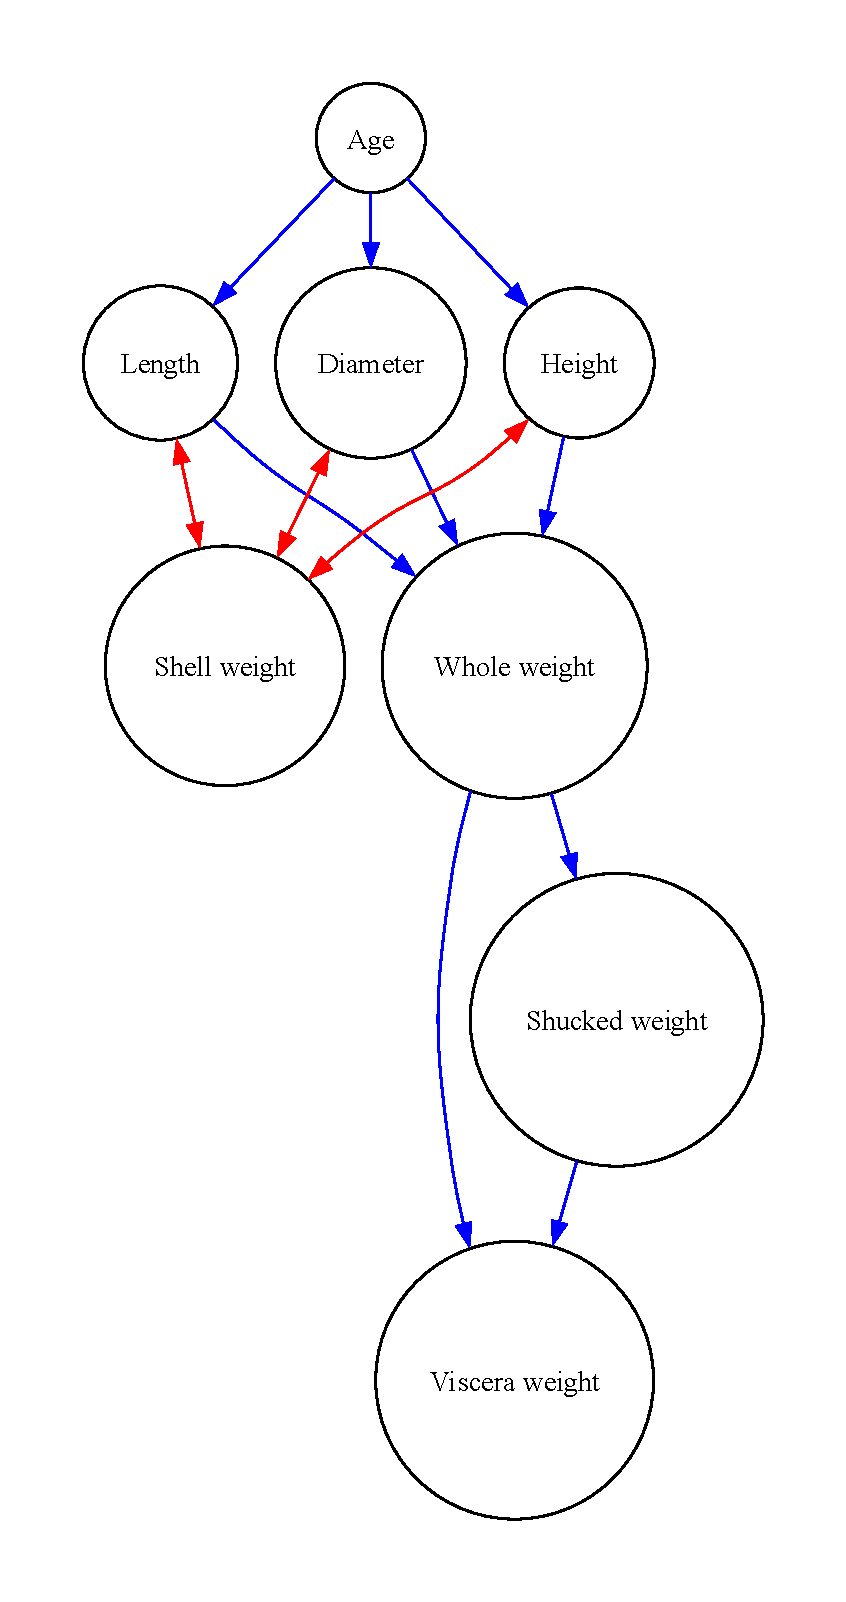
\includegraphics[height=0.4\textheight]{dataset/Abalone/output_graph/potential_relation.pdf}}
        \caption{\label{fig:relation}Possible Causal Relation Graph}
    \end{figure}
\end{minipage}

\section{Dataset Descriptions and EDA}
The following is a preview of our original dataset.

\begin{table}[H]
    \centering
    \caption{Dataset Preview}
    \begin{tabular}{rrrrrrrr}
\toprule
 Age &  Length &  Shell weight &  Diameter &  Height &  Whole weight &  Shucked weight &  Viscera weight \\
\midrule
15.0 &   0.455 &         0.365 &     0.095 &  0.5140 &        0.2245 &          0.1010 &           0.150 \\
 7.0 &   0.350 &         0.265 &     0.090 &  0.2255 &        0.0995 &          0.0485 &           0.070 \\
 9.0 &   0.530 &         0.420 &     0.135 &  0.6770 &        0.2565 &          0.1415 &           0.210 \\
10.0 &   0.440 &         0.365 &     0.125 &  0.5160 &        0.2155 &          0.1140 &           0.155 \\
 7.0 &   0.330 &         0.255 &     0.080 &  0.2050 &        0.0895 &          0.0395 &           0.055 \\
\bottomrule
\end{tabular}
\end{table}

\subsection{Data Properties}
We employ several statistical methods to identify data properties.

The shape of the data, data types, and missing values are assessed directly from the dataframe.
Linearity is evaluated using Ramsey’s RESET test, followed by the Benjamini \& Yekutieli procedure for multiple test correction.
Gaussian noise is assessed through the Shapiro-Wilk test, also applying the Benjamini \& Yekutieli procedure for multiple test correction.
Time-Series and Heterogeneity are derived from user queries.

Properties of the dataset we analyzed are listed below.

\begin{table}[H]
    \centering
    \caption{Data Properties}
    \begin{tabular}{rrrrrrr}
\toprule
Shape ($n$ x $d$) & Data Type & Missing Value & Linearity & Gaussian Errors & Time-Series & Heterogeneity \\
\midrule
(4177, 8)   & Continuous & False & False & False & False & False \\
\bottomrule
\end{tabular}
\end{table}

\subsection{Distribution Analysis}
The following figure shows distributions of different variables. The orange dash line represents the mean, 
and the black line represents the median. Variables are categorized into three types according to their distribution characteristics.

\begin{figure}[H]
\centering
\includegraphics[width=\linewidth]{dataset/Abalone/output_graph/eda_dist.jpg}
\caption{\label{fig:dist}Distribution Plots of Variables}
\end{figure}

\begin{itemize}
\item Slight left skew distributed variables: Length, Shell weight, Diameter, Whole weight
\item Slight right skew distributed variables: Age, Height, Shucked weight, Viscera weight
\item Symmetric distributed variables: None
\end{itemize}

\subsection{Correlation Analysis}

\begin{minipage}[t]{0.5\linewidth}
    In this analysis, we will categorize the correlation statistics of features in the dataset into three distinct categories: Strong correlations ($r>0.8$), Moderate correlations ($0.5<r<0.8$), and Weak correlations ($r<0.5$).

\begin{itemize}
\item Strong Correlated Variables: Shell weight and Length, Height and Whole weight, Shucked weight and Length, Viscera weight and Length, Viscera weight and Shell weight, Viscera weight and Height, Shucked weight and Height, Shucked weight and Whole weight
\item Moderate Correlated Variables: Length and Age, Shell weight and Age, Diameter and Age, Diameter and Length, Height and Age, Whole weight and Diameter, Shucked weight and Diameter, Viscera weight and Age, Viscera weight and Diameter, Viscera weight and Whole weight
\item Weak Correlated Variables: Shucked weight and Age
\end{itemize}
\vfill
\end{minipage}
\hfill
\begin{minipage}[t]{0.5\linewidth}
    \begin{figure}[H]
        \centering
        \vspace{-1.5cm}
        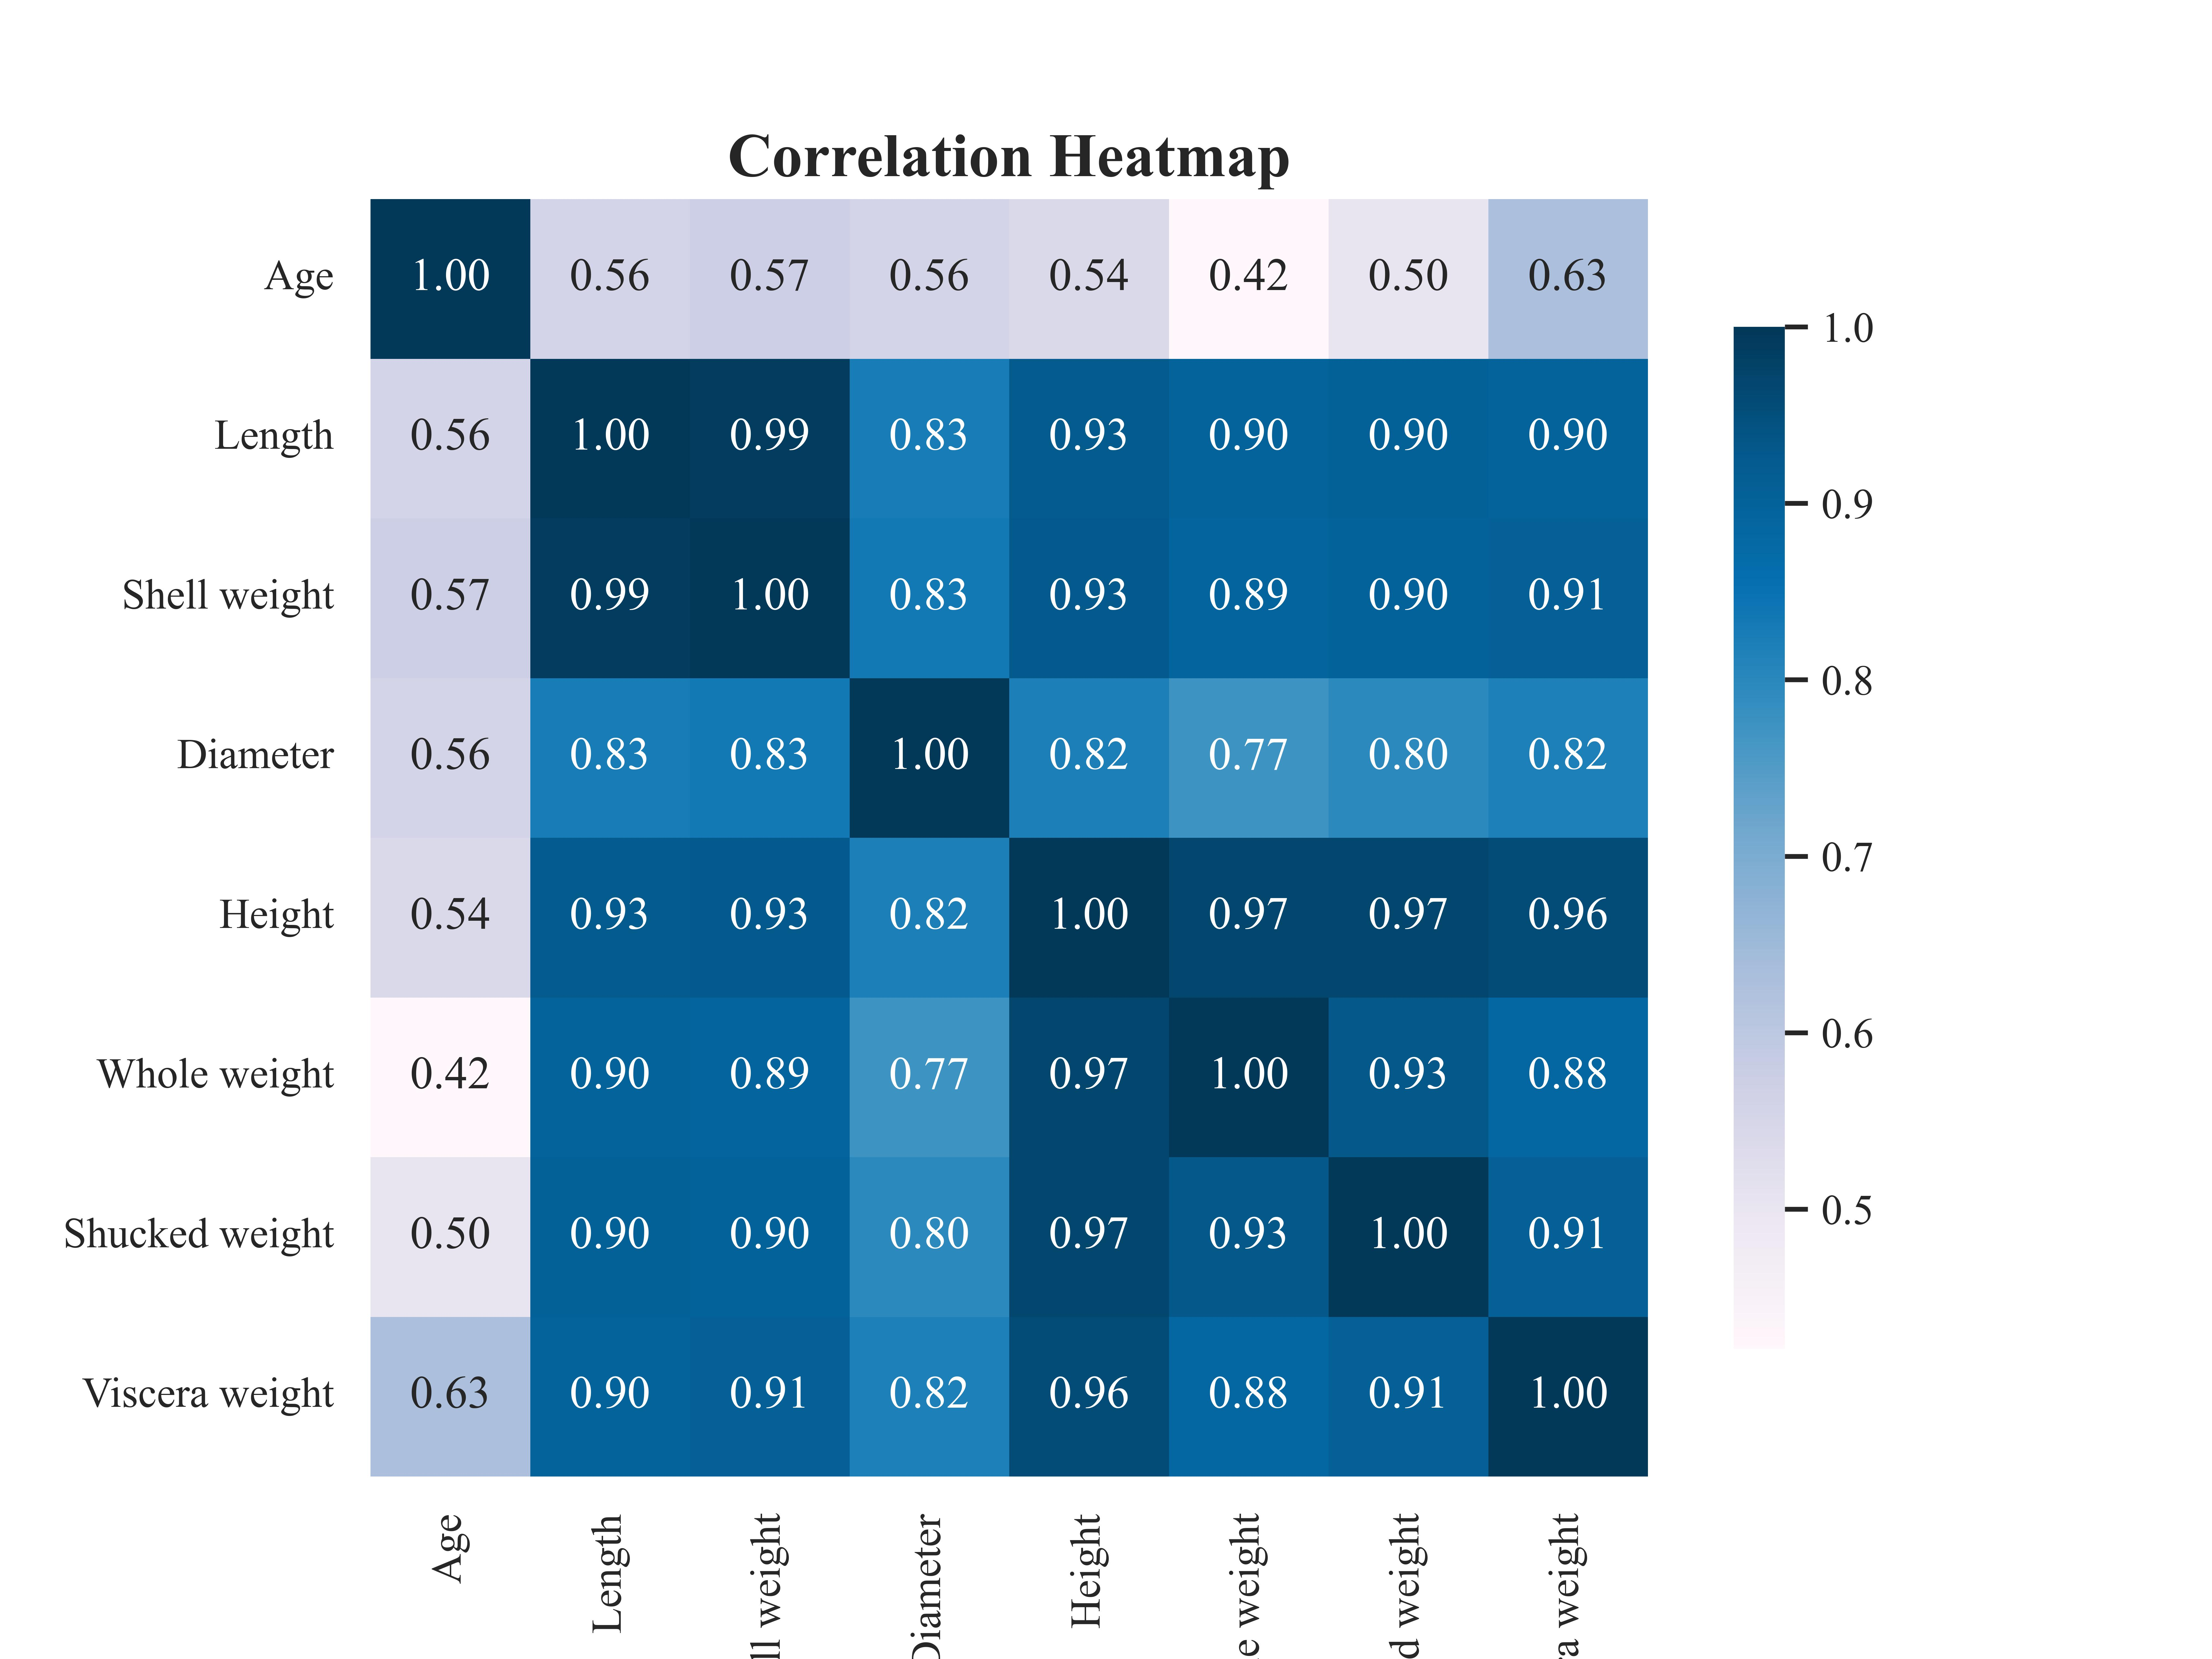
\includegraphics[width=\linewidth]{dataset/Abalone/output_graph/eda_corr.jpg}
        \caption{\label{fig:corr}Correlation Heatmap of Variables}
    \end{figure}
\end{minipage}

\section{Discovery Procedure}
In this section, we provide a detailed description of the causal discovery process implemented by Causal Copilot. 
We also provide the chosen algorithms and hyperparameters, along with the justifications for these selections.

\subsection{Data Preprocessing}
In this initial step, we preprocessed the data and examined its statistical characteristics. 
This involved cleaning the data, handling missing values, and performing exploratory data analysis to understand distributions and relationships between variables.

\subsection{Algorithm Selection assisted with LLM}
Following data preprocessing, we employed a large language model (LLM) to assist in 
selecting appropriate algorithms for causal discovery based on the statistical characteristics of the dataset and relevant background knowledge. 
The top three chosen algorithms, listed in order of suitability, are as follows:   

\begin{itemize}

    \item \textbf{PC}:
    \begin{itemize}
        \item \textbf{Description}: The PC algorithm is a constraint-based method that learns the structure of a causal graph from data by testing conditional independencies between variables, constructing a Directed Acyclic Graph (DAG).
        \item \textbf{Justification}: Given the large sample size of 4177 and the presence of all relevant observed variables, the PC algorithm is a strong candidate for discovering causal relationships despite the non-linear nature of the dependencies.
    \end{itemize}

    \item \textbf{GES}:
    \begin{itemize}
        \item \textbf{Description}: Greedy Equivalence Search (GES) is a score-based algorithm that identifies the optimal causal structure by navigating through equivalence classes of Directed Acyclic Graphs (DAGs) using a scoring function.
        \item \textbf{Justification}: Considering the dataset’s characteristics of having many continuous variables but no missing data, GES provides an efficient method for navigation in the complex structure, accommodating the non-Gaussian distributions while maintaining computational efficiency.
    \end{itemize}

    \item \textbf{NOTEARS}:
    \begin{itemize}
        \item \textbf{Description}: NOTEARS transforms the combinatorial problem of learning Directed Acyclic Graphs (DAGs) into a continuous optimization problem, allowing it to efficiently scale to large datasets.
        \item \textbf{Justification}: Though it assumes linear causality, NOTEARS can handle the dataset's continuous nature and is suitable for high-dimensional settings, making it a viable option for exploring causal relationships in this dataset.
    \end{itemize}

\end{itemize}

\subsection{Hyperparameter Values Proposal assisted with LLM}
Once the algorithms were selected, the LLM aided in proposing hyperparameters 
for the algorithm, which are specified below:

\begin{itemize}

    \item \textbf{alpha}:
    \begin{itemize}
        \item \textbf{Value}: 0.05
        \item \textbf{Explanation}: The default value of 0.05 is appropriate given that the sample size is sufficiently large (4177), which allows for a balance between reducing false positives while still being moderately conservative. Lowering it would reduce the chance of detecting true causal relationships.
    \end{itemize}

    \item \textbf{indep\_test}:
    \begin{itemize}
        \item \textbf{Value}: fisherz
        \item \textbf{Explanation}: Fisher's Z test is appropriate here since the data is continuous. Despite the fact that the relationships may not be predominantly linear and the errors do not follow a Gaussian distribution, Fisher's Z test is still commonly used for continuous data due to its straightforward implementation and efficiency.
    \end{itemize}

    \item \textbf{depth}:
    \begin{itemize}
        \item \textbf{Value}: -1
        \item \textbf{Explanation}: Using the default value of -1 allows the PC algorithm to explore the full depth of the graph structure without artificially limiting the exploration. This maximizes the algorithm's ability to find all potential causal relations present in the data.
    \end{itemize}

\end{itemize}

\subsection{Graph Tuning with LLM Suggestion}
In the final step, we performed graph tuning with suggestions provided by the LLM.
We utilized LLM to help us determine the direction of undirected edges according to its knowledge repository.
By integrating insights from the LLM to refine the causal graph, we can achieve improvements in graph's accuracy and robustness.

\begin{itemize}
    \item \textbf{Height $\rightarrow$ Whole weight}: As the height of abalones increases, their whole weight is likely to increase as well due to overall growth, indicating that height can influence whole weight.

    \item \textbf{Length $\rightarrow$ Shell weight}: A larger length in abalones typically correlates with a heavier shell, suggesting that length is a causal factor for shell weight.
\end{itemize}

This structured approach ensures a comprehensive and methodical analysis of the causal relationships within the dataset.

\section{Results Summary}

\begin{figure}[H]
    \centering
    \begin{subfigure}{0.3\textwidth}
        \centering
        \vspace{-0.5cm}
        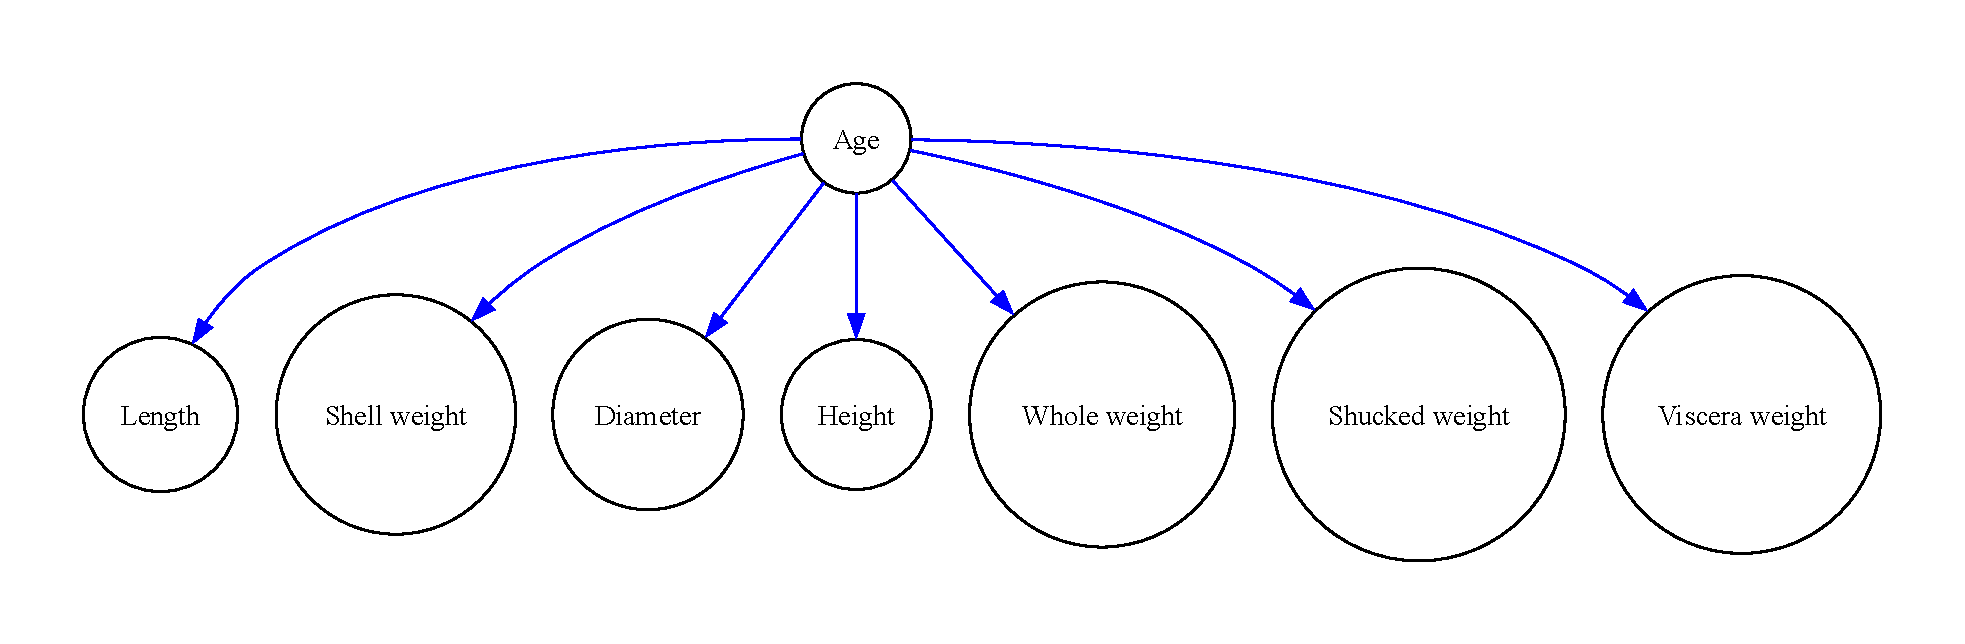
\includegraphics[width=\linewidth]{dataset/Abalone/output_graph/true_graph.pdf}
        \vfill
        \caption{True Graph}
        \label{fig:sub1}
    \end{subfigure}
    \hspace{0.04\textwidth}
    \begin{subfigure}{0.3\textwidth}
        \centering
        \vspace{-0.5cm}
        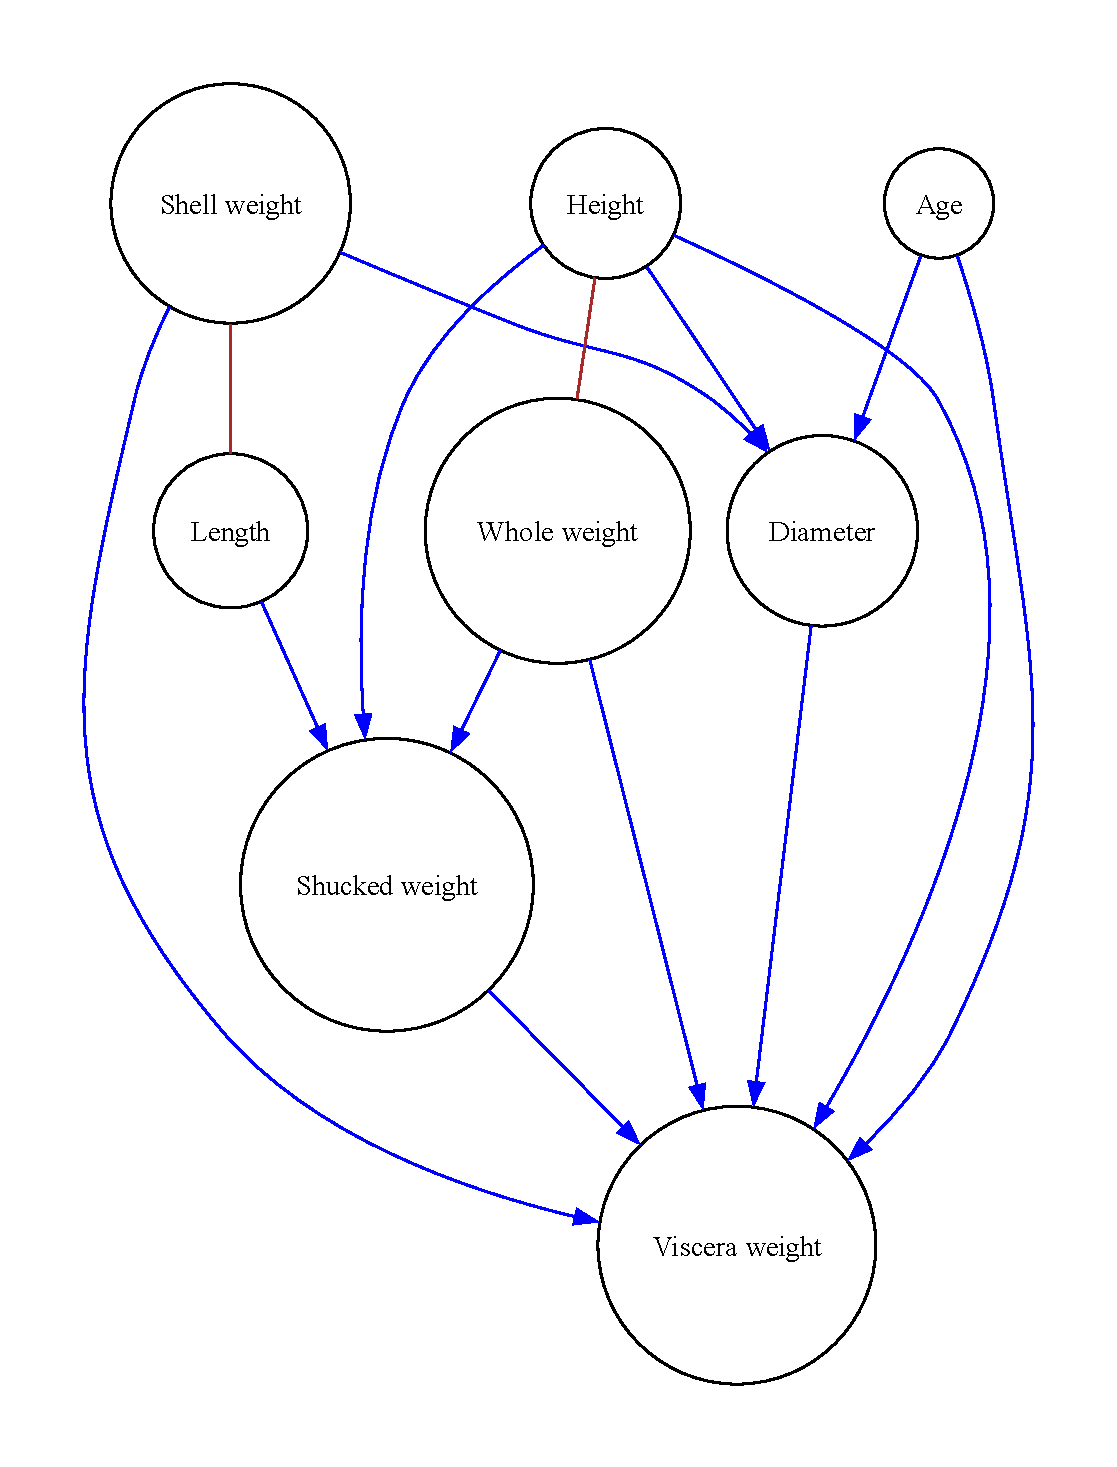
\includegraphics[width=\linewidth]{dataset/Abalone/output_graph/initial_graph.pdf}
        \vfill
        \caption{Initial Graph}
        \label{fig:sub2}
    \end{subfigure}
    \hspace{0.04\textwidth}
    \begin{subfigure}{0.3\textwidth}
        \centering
        \vspace{-0.5cm}
        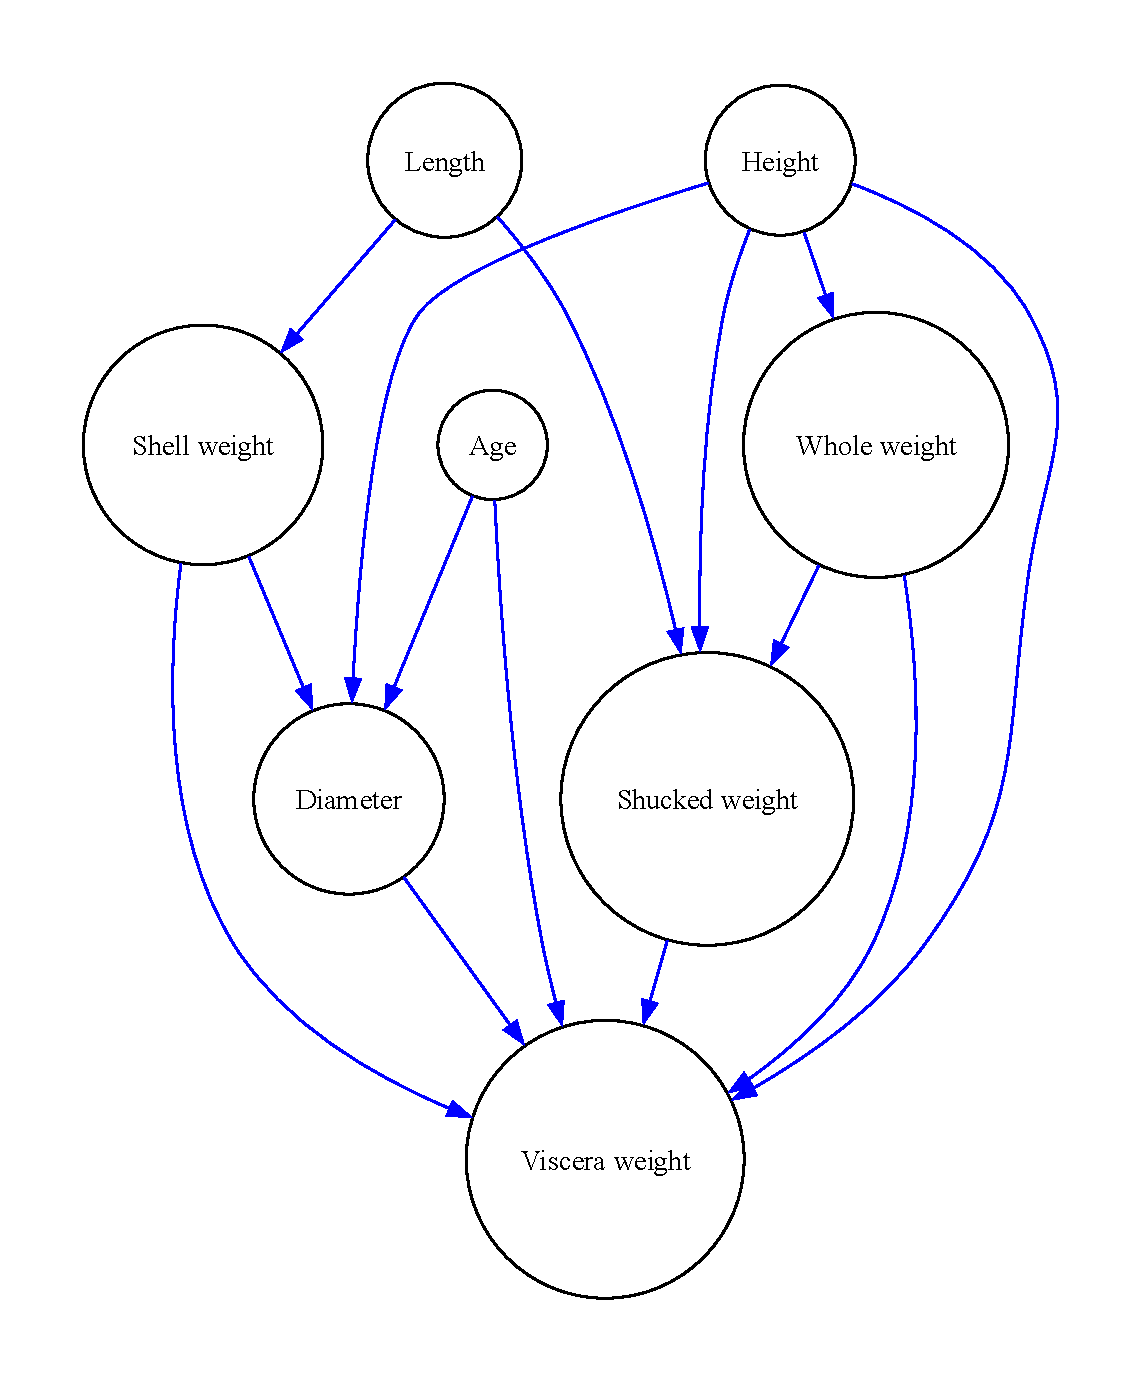
\includegraphics[width=\linewidth]{dataset/Abalone/output_graph/revised_graph.pdf}
        \vfill
        \caption{Revised Graph}
        \label{fig:sub3}
    \end{subfigure}
    \caption{Graphs Comparison of PC}
    \label{fig:main}
\end{figure}

The above are result graphs produced by our algorithm.
The initial graph is the graph in the first attempt, and the revised graph is the one pruned with LLM suggestion.

The analysis of causal relationships among the variables reveals a complex interplay where Age influences both Diameter and Viscera weight, suggesting that as organisms mature, their body structures and internal mass increase. Length not only affects Shell weight but also Shucked weight, indicating that greater lengths are associated with heavier shells and more substantial meat content. Additionally, Shell weight reciprocally influences Length and extends its impact to Diameter and Viscera weight, highlighting its central role in determining both the physical dimensions and biological mass of the organism. Height appears to be a significant factor as it drives changes in Diameter, Whole weight, Shucked weight, and Viscera weight, reflecting the overall growth dynamics. Whole weight, in turn, affects Height, Shucked weight, and Viscera weight, suggesting that larger overall mass contributes to broader physiological changes. Finally, Shucked weight has a direct causal effect on Viscera weight, indicating its relevance in determining the internal mass of the organism. Overall, the intricate relationships among these variables underscore the biological principles of growth and development within the organism.

\subsection{Graph Reliability Analysis}

\begin{figure}[H]
    \centering
    \vspace{-0.5cm}
    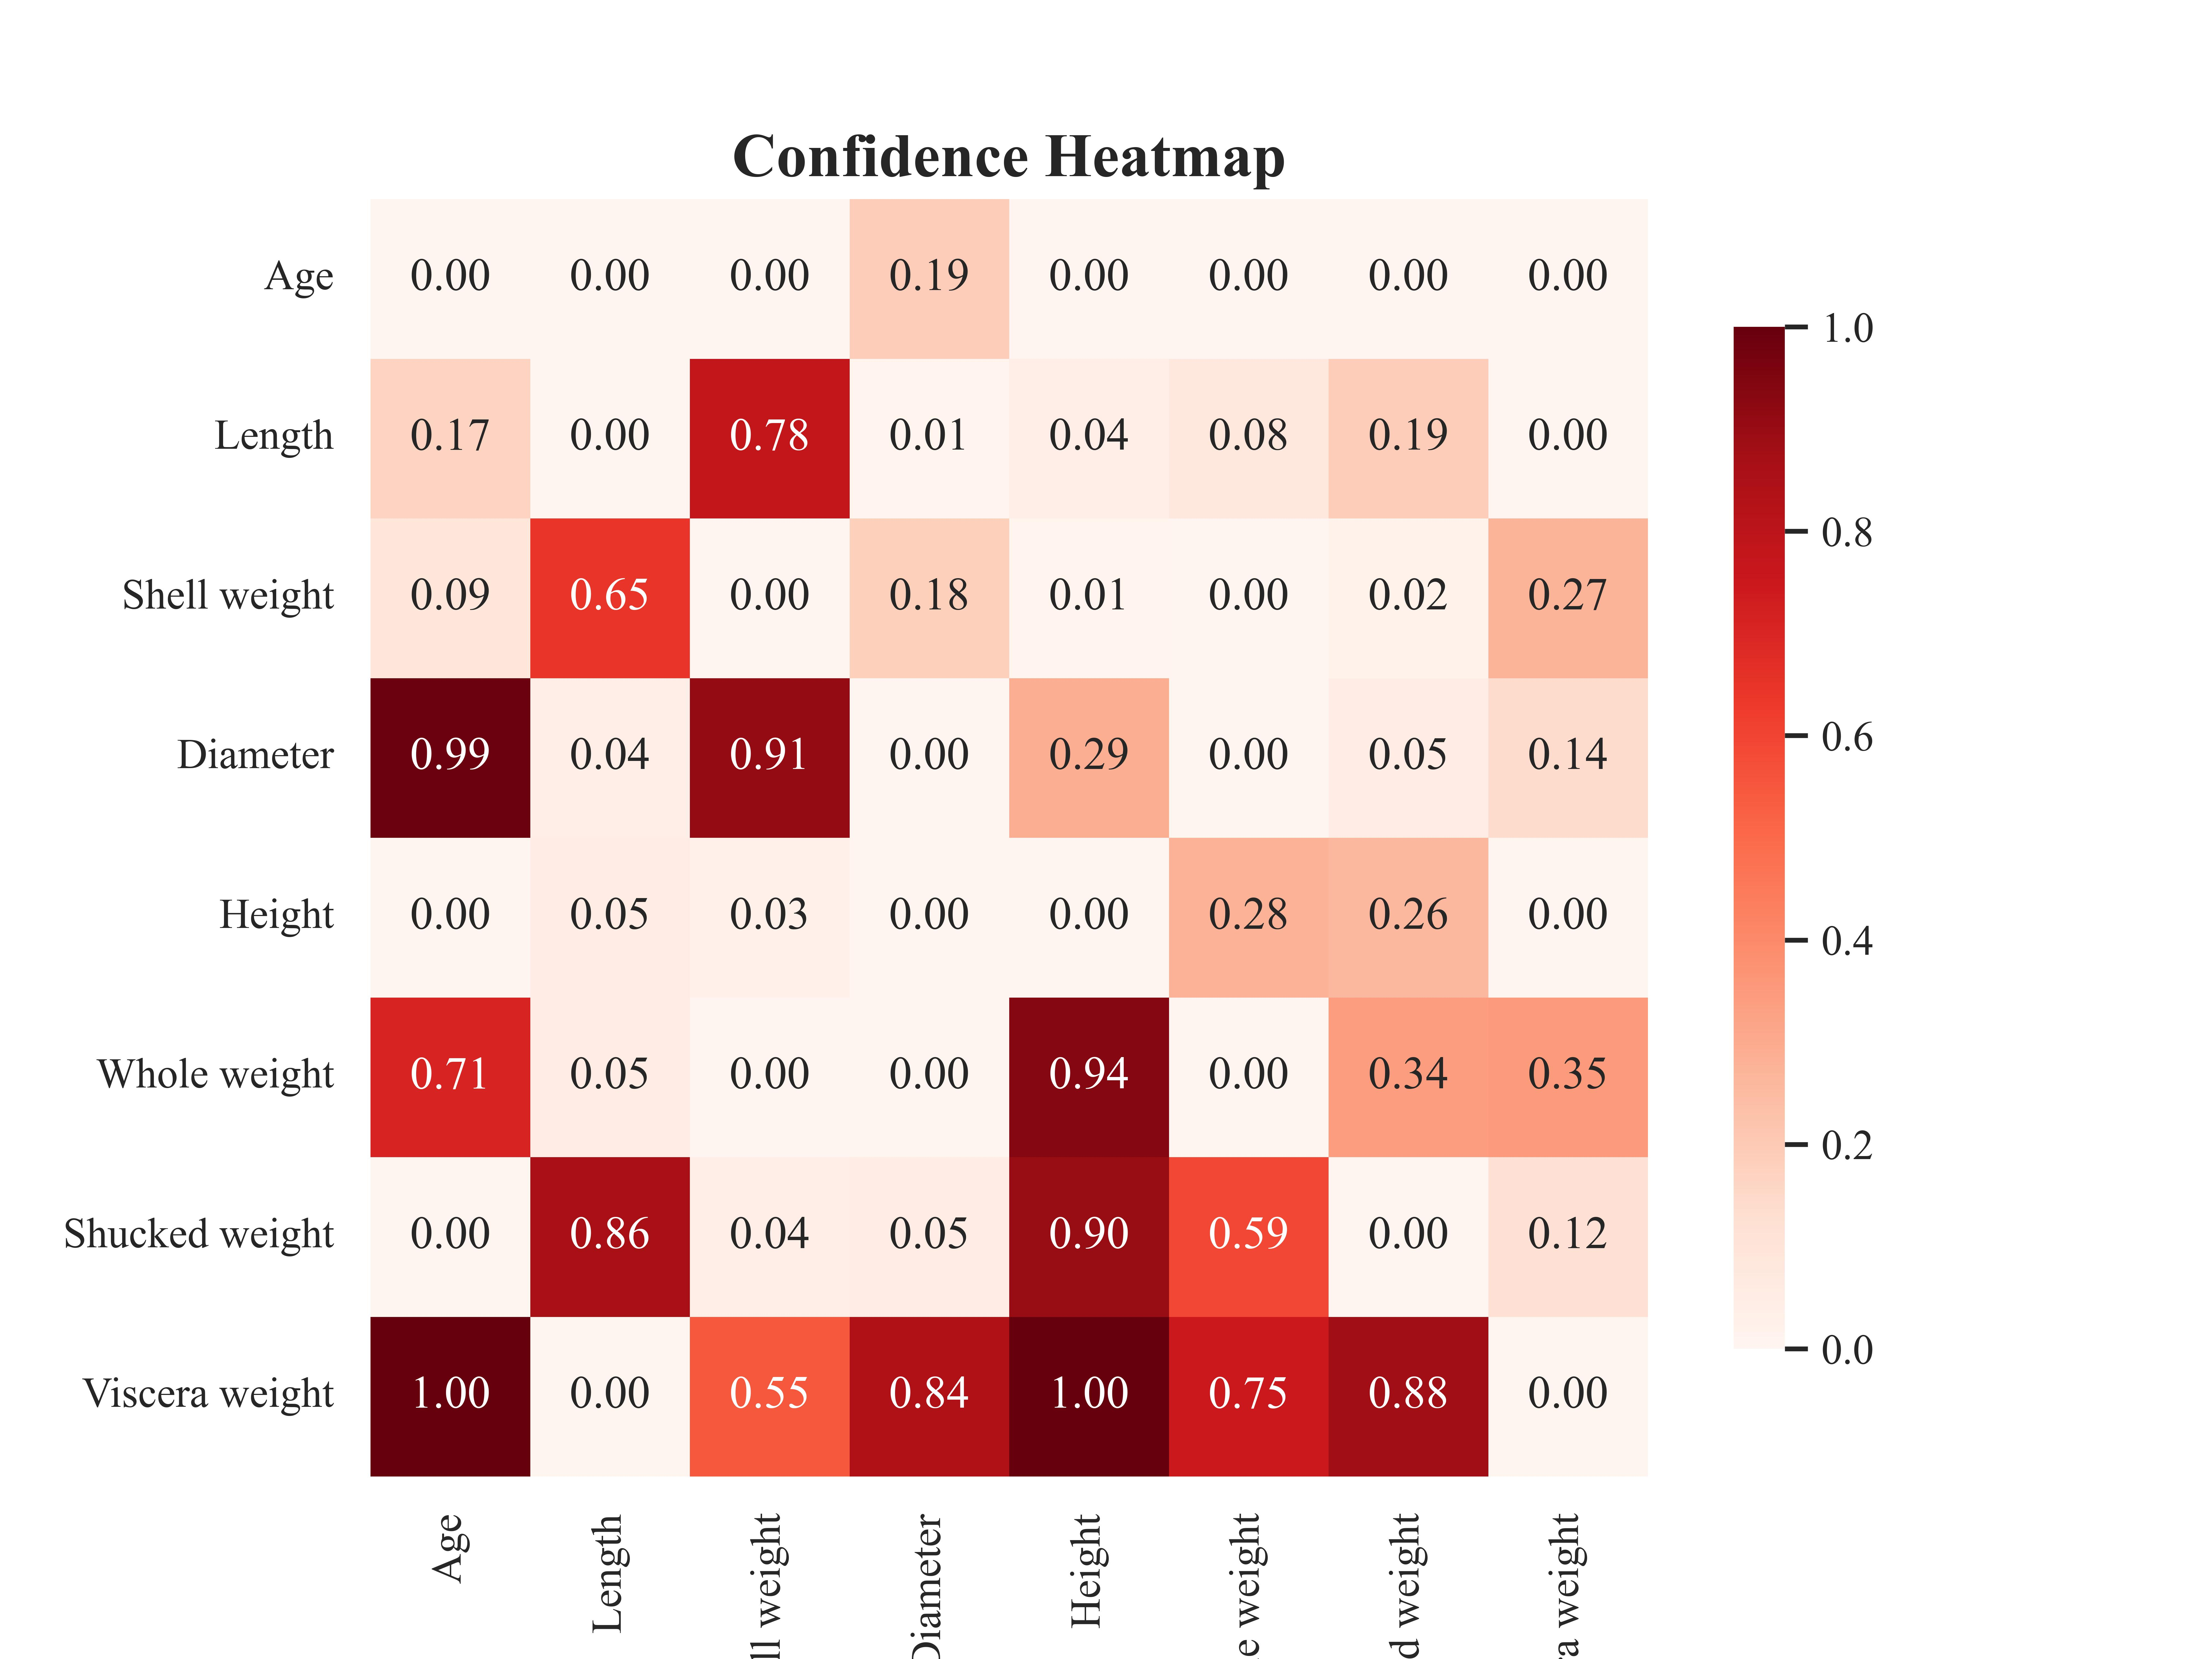
\includegraphics[width=0.8\linewidth]{dataset/Abalone/output_graph/confidence_heatmap.jpg}
    \caption{Reliability Graph}
    \label{fig:sub3}
\end{figure}

Based on the confidence probability heatmap and background knowledge, we can analyze the reliability of our graph.

From the statistics perspective, we have high confidence to believe that the edges Length $\rightarrow$ Shell weight (bootstrap probability of 0.78) and Whole weight $\rightarrow$ Height (bootstrap probability of 0.94) exist, indicating a strong causal relationship. Conversely, we have low confidence in the edges Age $\rightarrow$ Diameter (0.19) and Age $\rightarrow$ Viscera weight (0.0), as well as Height $\rightarrow$ Diameter (0.0) and Height $\rightarrow$ Viscera weight (0.0), suggesting these edges are likely not present. 

However, based on expert knowledge, we know that the edges Age $\leftrightarrow$ Length, Diameter, and Height are likely to exist due to the biological growth patterns seen in abalones, where increasing age typically correlates with larger physical dimensions. Moreover, the relationships between Whole weight and both Shucked weight and Viscera weight are supported by the understanding that heavier abalones generally produce more meat and have more substantial viscera. 

Therefore, the result of this causal graph is partially reliable. While some relationships indicated by the bootstrap probabilities align with expert knowledge, other edges defined as likely non-existent by the bootstrap results conflict with established biological insights. This discrepancy highlights the need for further investigation and additional data to refine the causal relationships among these variables.

\end{document}